\section{Fundamentals about Image}
\begin{frame}<beamer>
    \frametitle{Outline}
    \tableofcontents[currentsection]
\end{frame}

\begin{frame}
 \frametitle{Opening Discussion (1)}
 \begin{itemize}
 	\item {From now on, we are going to explore a new field}
 	\item {Image and Videos}
 	\item {It is another dimension of Multimedia}
 	\item {In our daily life, around \textbf{80\%} information comes from vision}
 	\item {With the proliferation of digital devices, millions of images/videos are generated each day}
 \end{itemize}
 \begin{figure}
 \begin{center}
	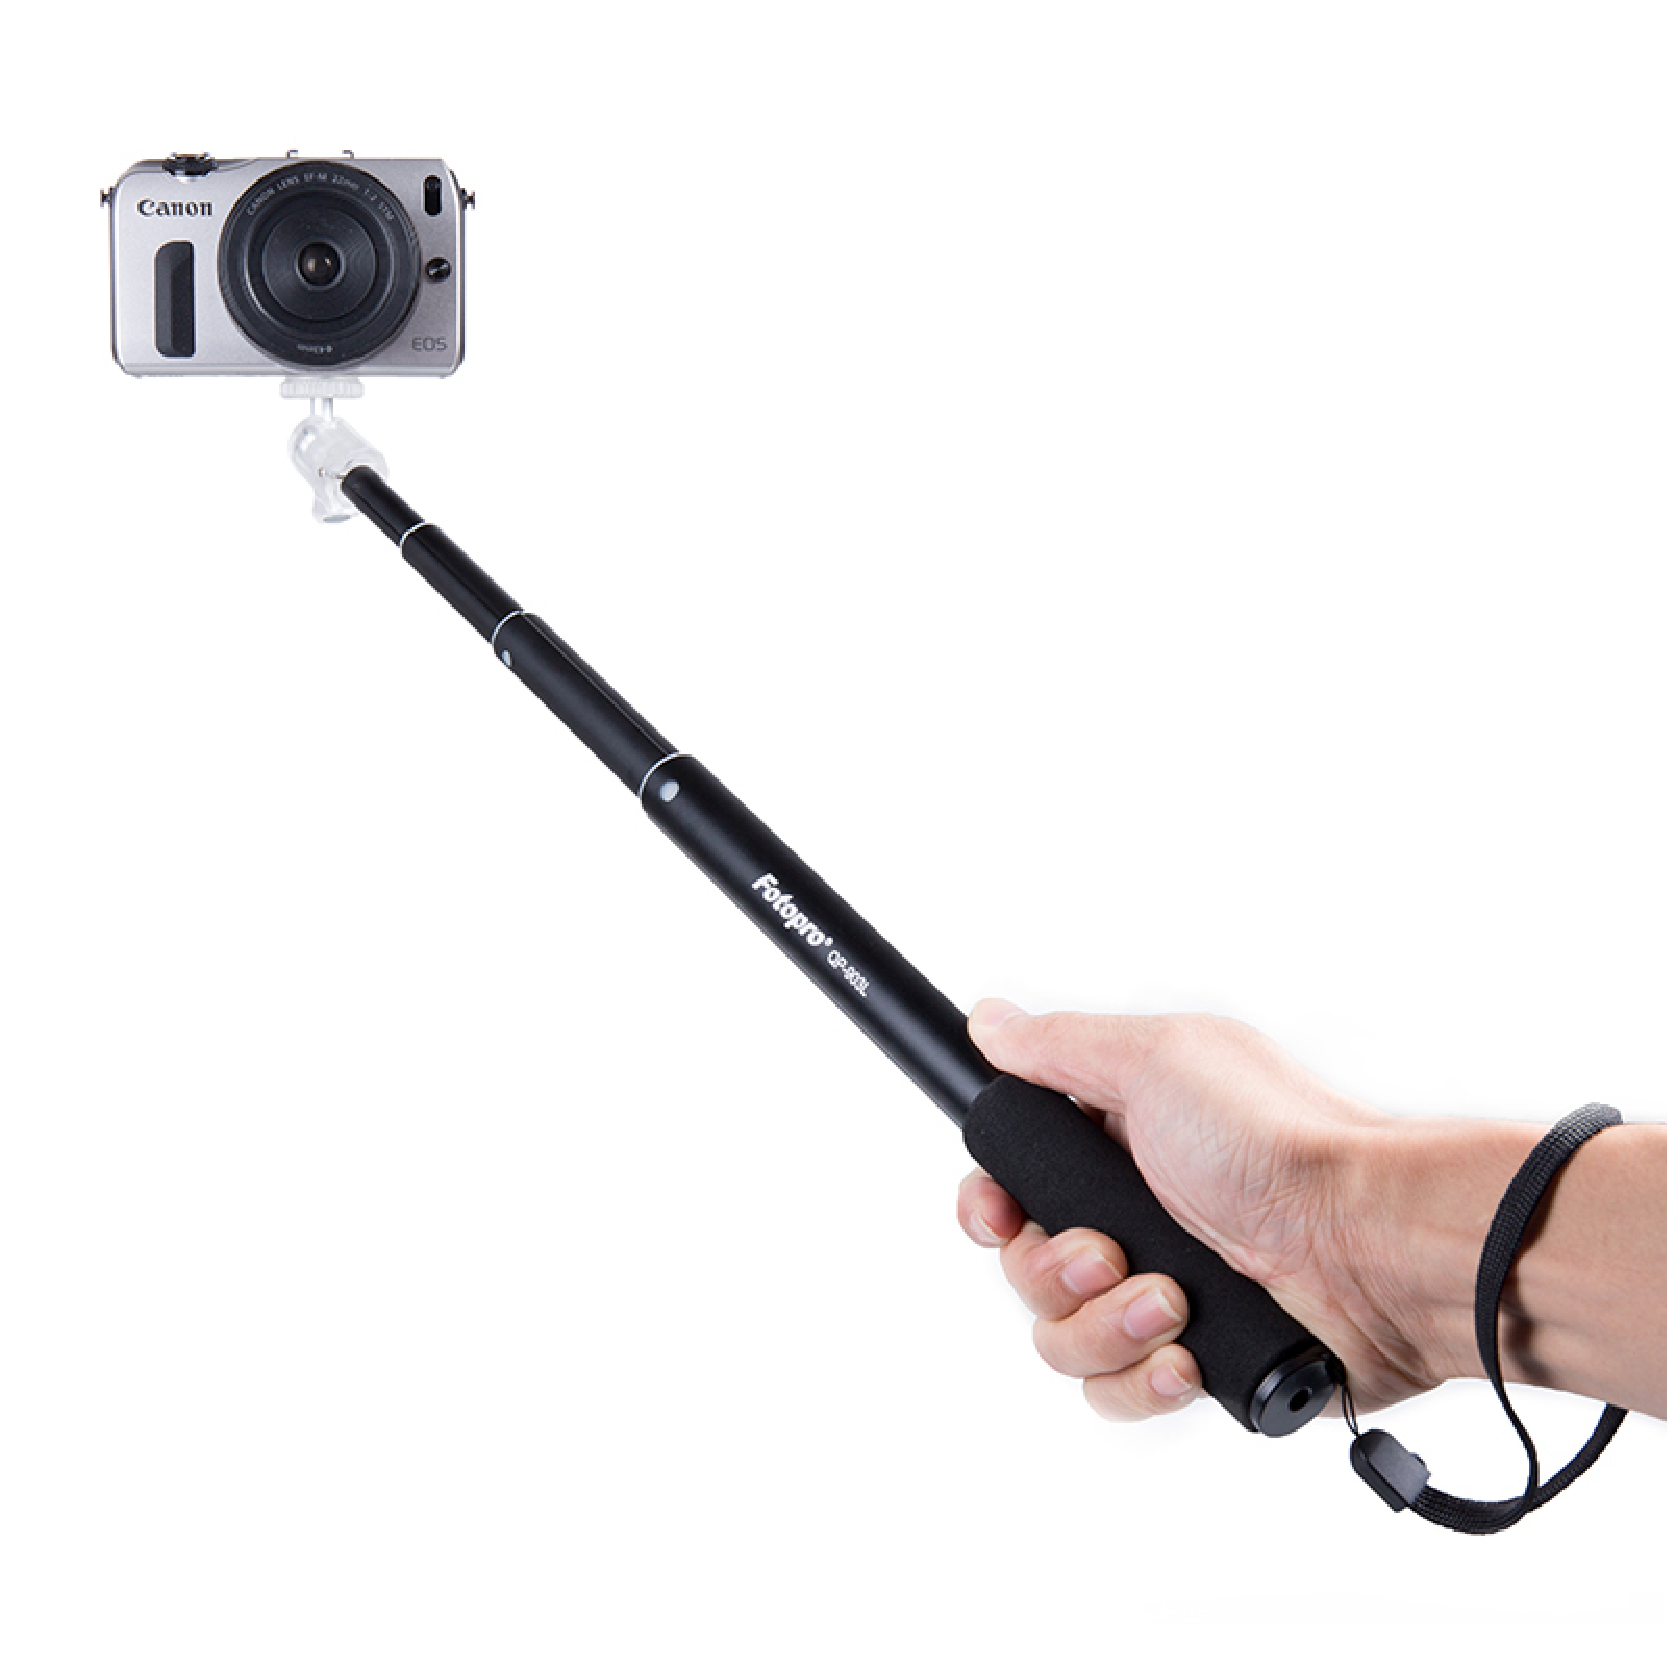
\includegraphics[width=0.350\linewidth]{./figs/support.pdf}
 \end{center}
 \end{figure}
\end{frame}
 
\begin{frame}
 \frametitle{Opening Discussion (2)}
\begin{itemize}
 	\item {It was \textcolor{red}{guessed} that vision caused \textbf{Cambrian Explosion} which took place in 542 million years ago}
 	\item {Vision drove all creatures to evolve faster to survive}
 	\item {With vision, they could search for food easier than before}
 \end{itemize} 
 \begin{figure}
\begin{center}
	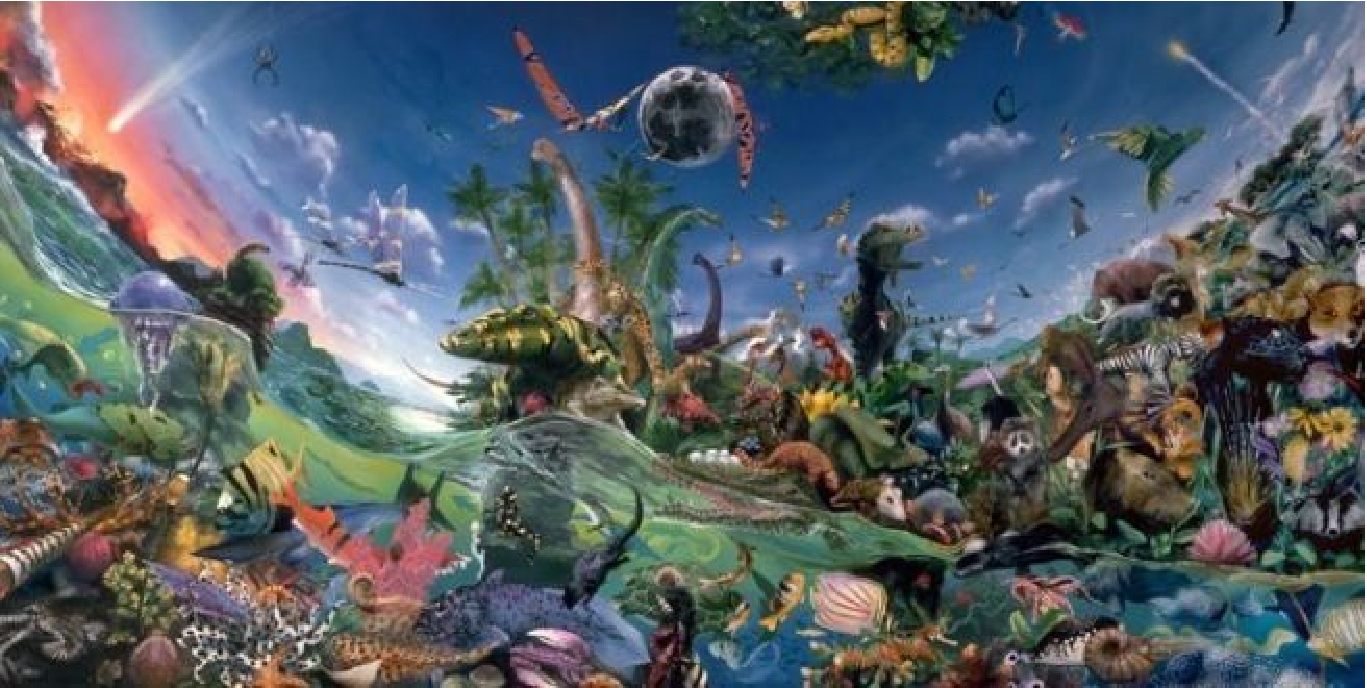
\includegraphics[width=0.80\linewidth]{./figs/cambrian.pdf}
\end{center}
\end{figure}

\end{frame}

\begin{frame}
 \frametitle{Brief history about Digital Image (1)}
 \begin{itemize}
 	\item {It was a long dream that one day we could keep what we see in somewhere besides our brain}
 \end{itemize}
 \begin{figure}
\begin{center}
	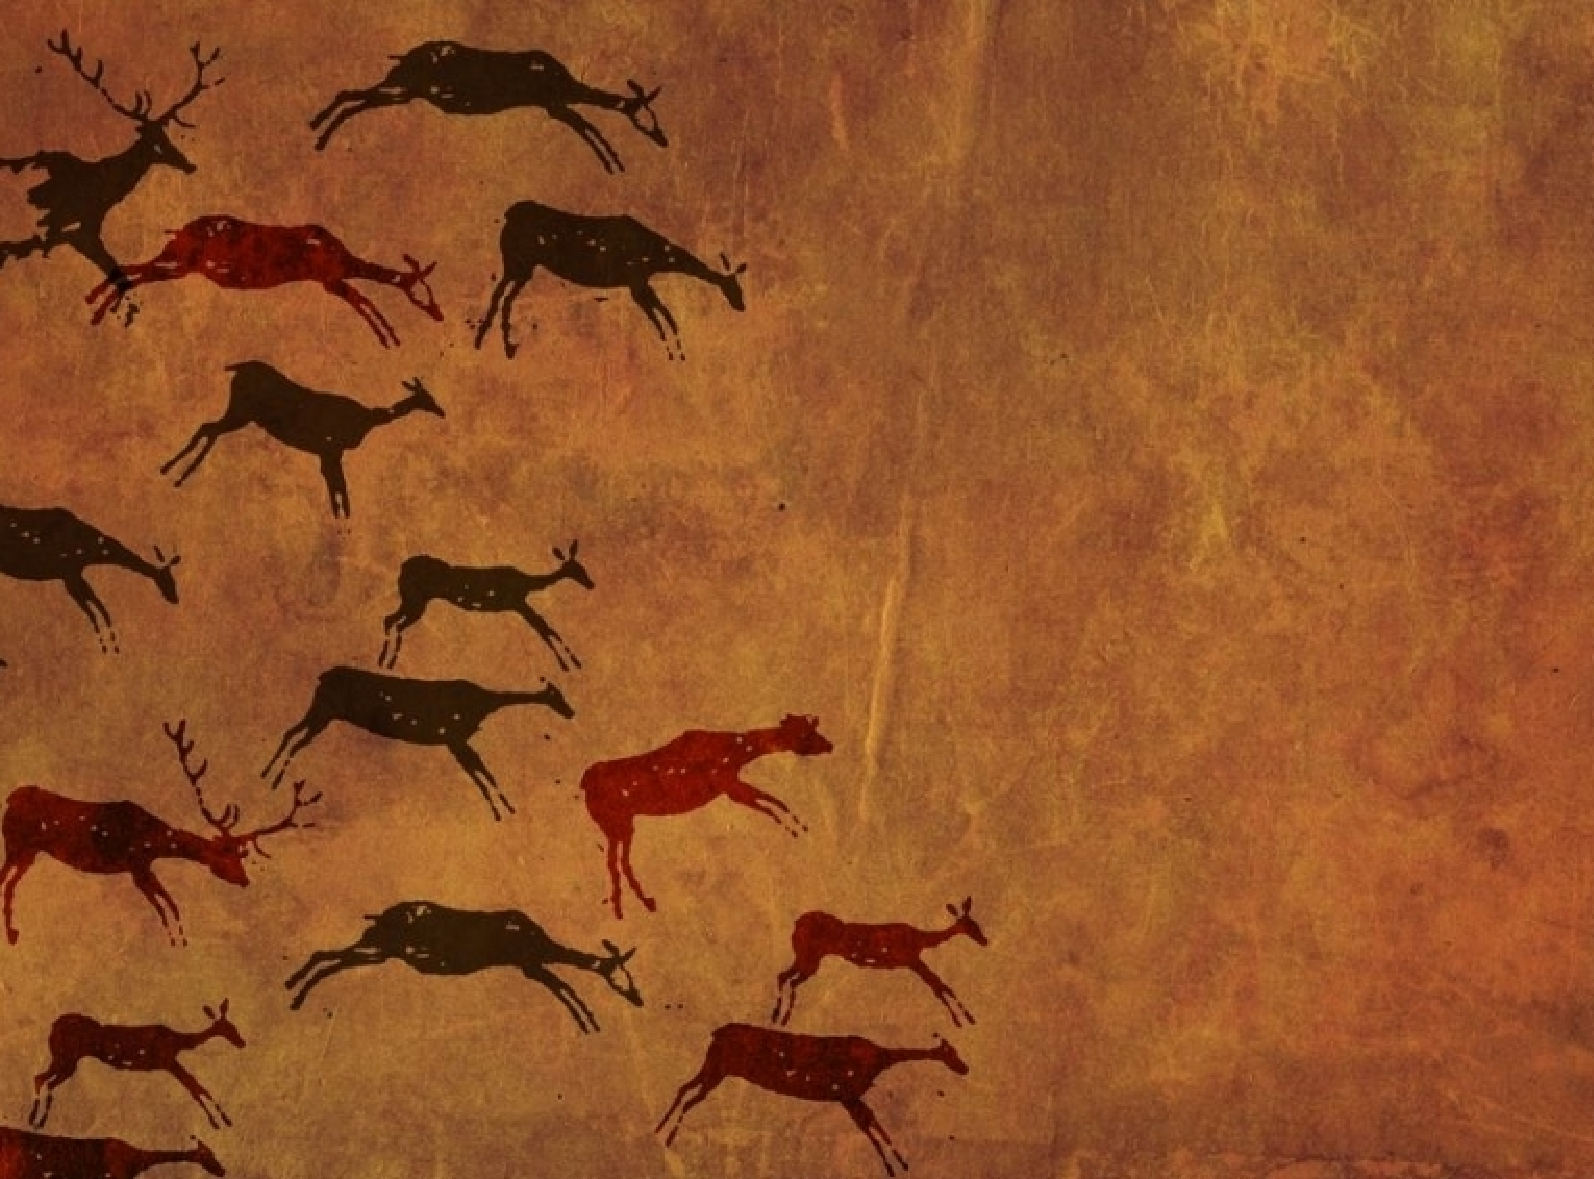
\includegraphics[width=0.6\linewidth]{./figs/neanderthal_paint.pdf}
\end{center}
\caption{Painting by Neanderthal who lived in Europe around 40,000 years ago.}
\end{figure}
\end{frame}

\begin{frame}
 \frametitle{Brief history about Digital Image (2)}
 \vspace{-0.1in}
 \begin{figure}
\begin{center}
	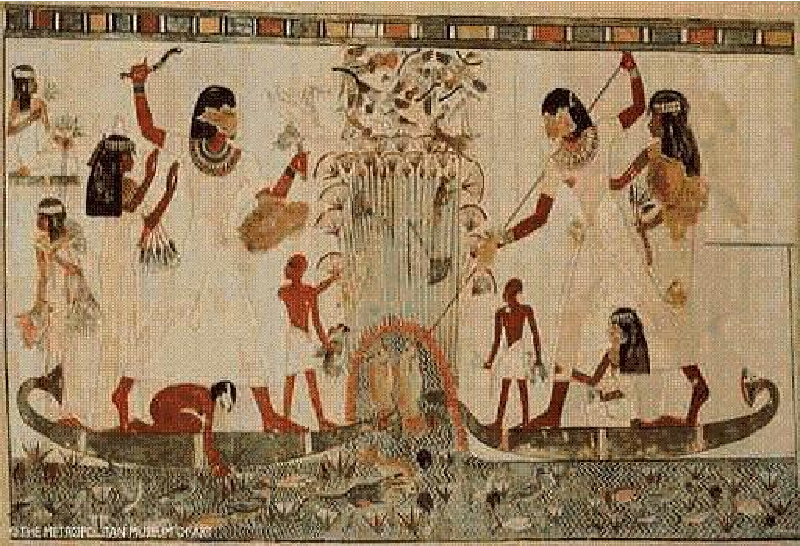
\includegraphics[width=0.66\linewidth]{./figs/egypt_paint.pdf}
\end{center}
\caption{Painting by ancient Egyptian who lived in 5,000 years ago.}
\end{figure}
 \begin{itemize}
 	\item {Notice that in these two periods, people could only try to draw what they saw}
 \end{itemize}
\end{frame}

\begin{frame}
 \frametitle{Brief history about Digital Image (3)}
 \begin{figure}
\begin{center}
	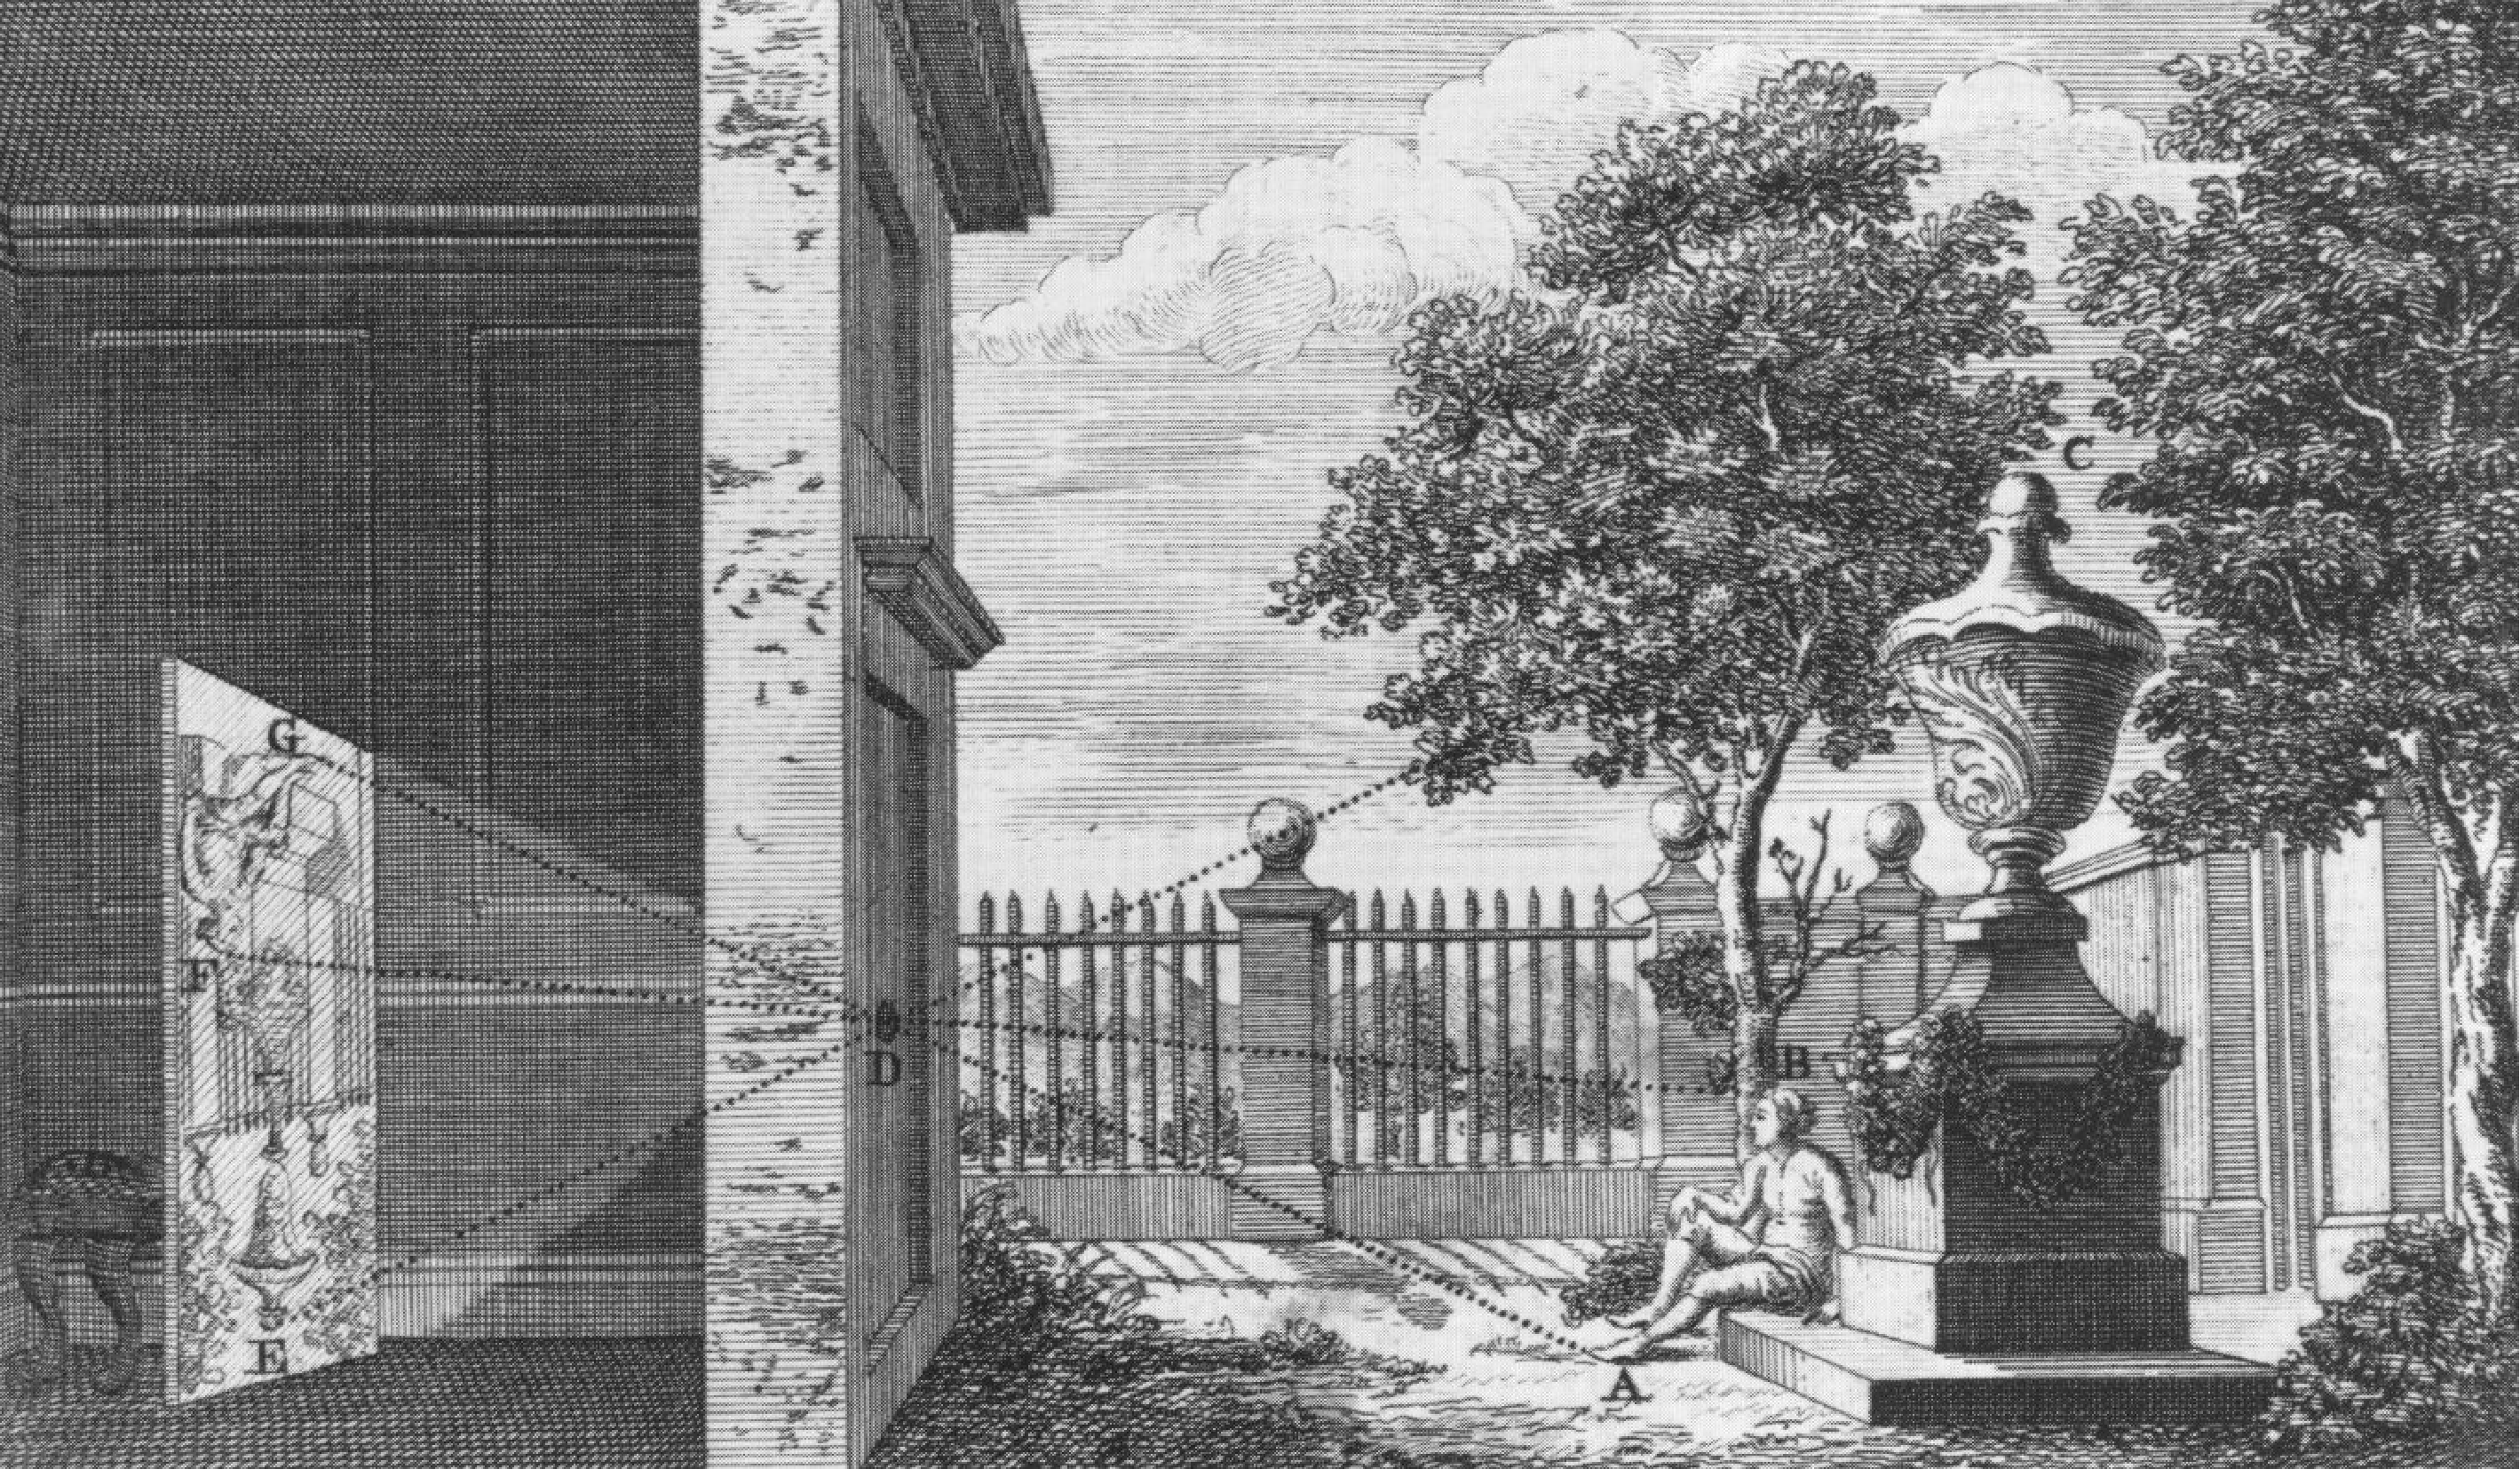
\includegraphics[width=0.66\linewidth]{./figs/camera_obscura.pdf}
\end{center}
\caption{The known first camera by Aristotle.}
\end{figure}
 \begin{itemize}
 	\item {Why it works?}
 	\item {How the size of aperture impacts the projected image}
 	\item {How to keep this capture is still a big problem}
 \end{itemize}
\end{frame}

\begin{frame}
 \frametitle{Brief history about Digital Image (4)}
\vspace{-0.1in}
\begin{figure}
\begin{center}
	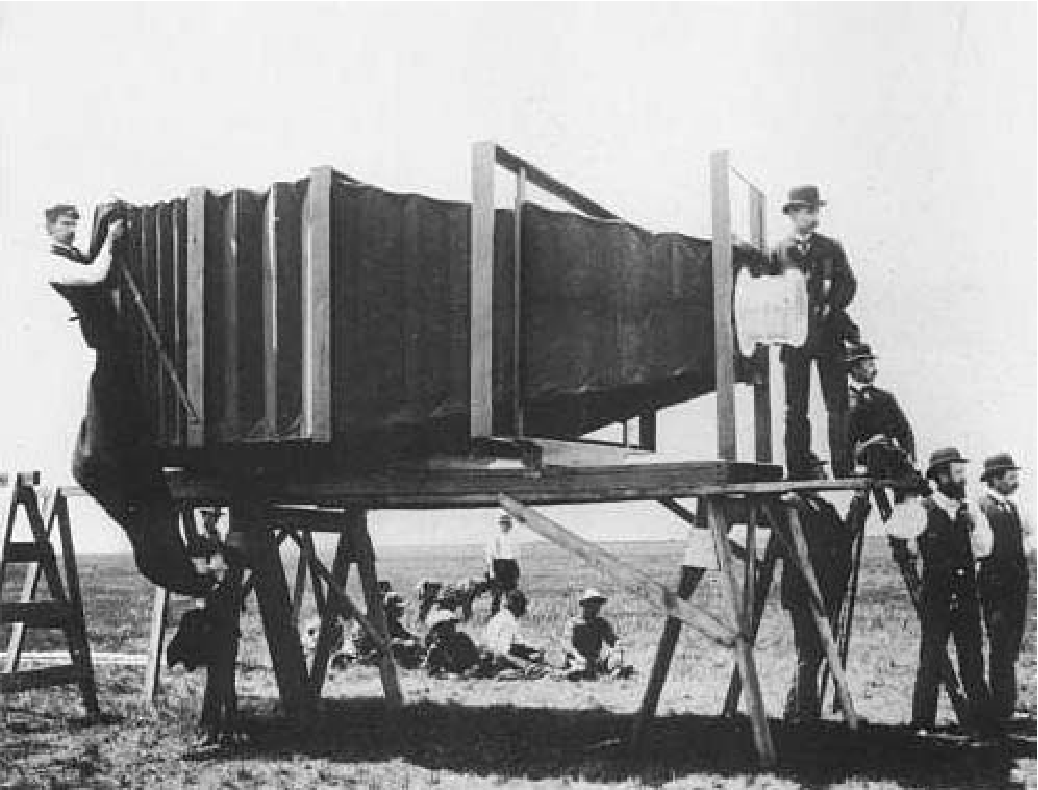
\includegraphics[width=0.53\linewidth]{./figs/biggest_camera.pdf}
\end{center}
\caption{In 1900 the Chicago \& Alton Railroad Train co. , commissioned Lawrence with the manufacture of the largest camera ever made and the largest photo ever shot in order to promote a new train.}
\end{figure}
\vspace{-0.1in}
\begin{itemize}
	\item {Around 30 years before that event, film was invented}
	\item {However, it requires long time of exposure}
\end{itemize}
\end{frame}

\begin{frame}
 \frametitle{Basic knowledge about camera}
  \vspace{-0.1in}
\begin{figure}
\begin{center}
	{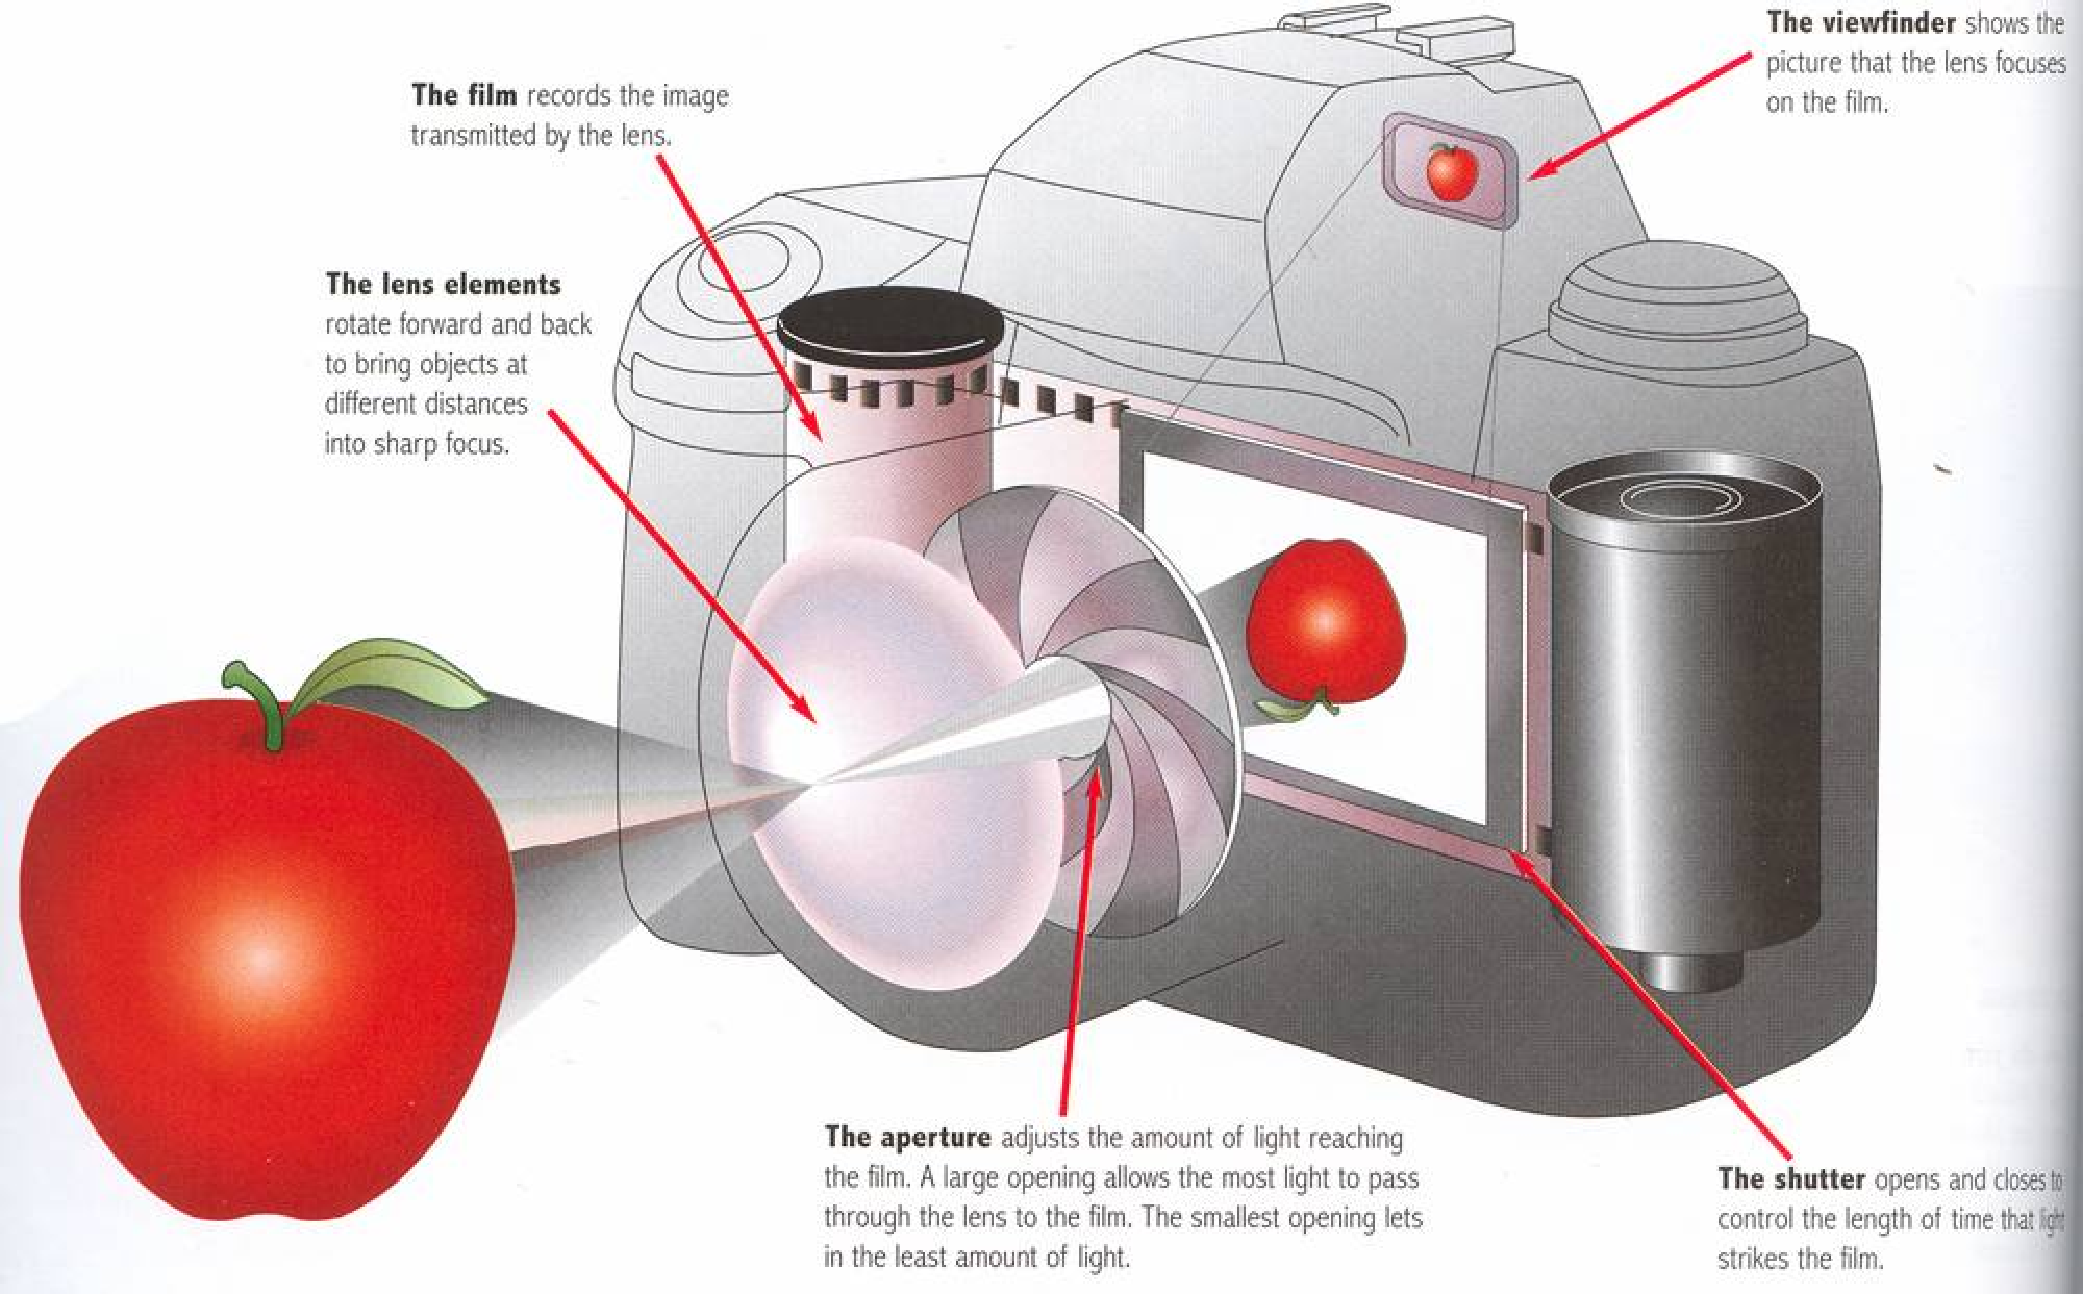
\includegraphics[width=0.55\linewidth]{./figs/camera.pdf}}
\end{center}
\caption{Structure of a modern camera}
\end{figure}

\begin{itemize}
	\item {Major components}
	\begin{enumerate}
		\item {Lens}
		\item {Aperture}
		\item {Film/Sensor field}
	\end{enumerate}
\end{itemize}

\end{frame}


\begin{frame}
 \frametitle{Basic knowledge about camera: the lens (1)}
  \vspace{0.2in}
\begin{figure}
\begin{center}
	{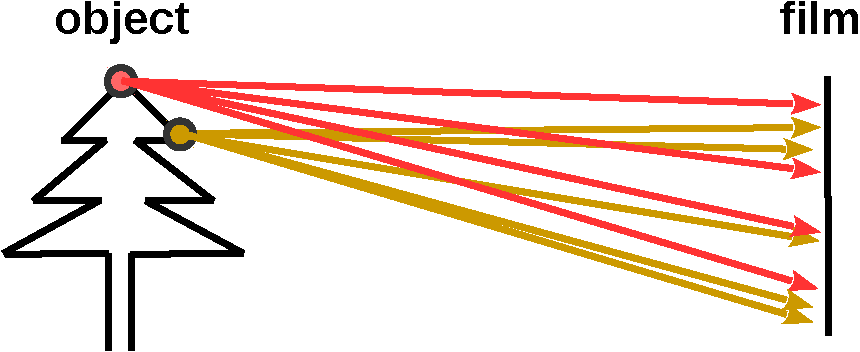
\includegraphics[width=0.5\linewidth]{./figs/holeno.pdf}}
\end{center}
\caption{Try to put film in front of an object, see what you can get}
\end{figure}
\begin{itemize}
	\item {You get nothing but gray because ambient lights come from all directions}
\end{itemize}
\end{frame}


\begin{frame}
 \frametitle{Basic knowledge about camera: the lens (2)}
  \vspace{-0.1in}
\begin{columns}
\begin{column}{0.35\linewidth}
\begin{figure}
\begin{center}
	{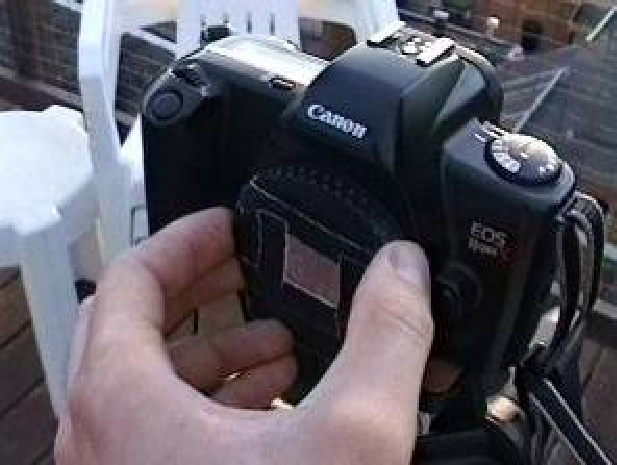
\includegraphics[width=0.75\linewidth]{./figs/removelens.pdf}}
\end{center}
\caption{Remove camera lens}
\end{figure}
\begin{itemize}
	\item {Why blurry??}
\end{itemize}
\end{column}
\begin{column}{0.65\linewidth}
\begin{figure}
\begin{center}
	{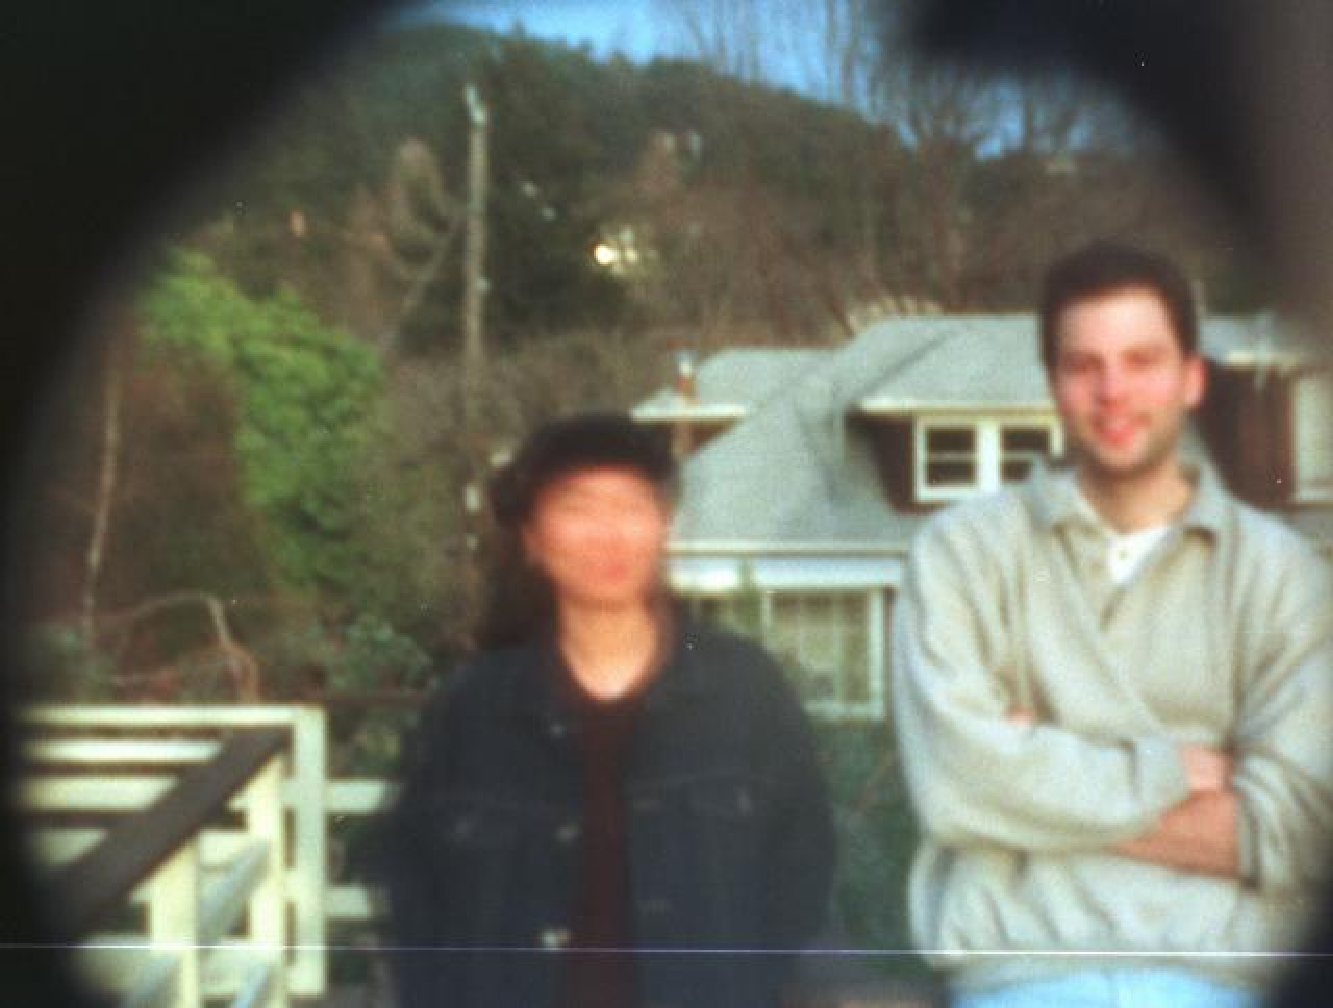
\includegraphics[width=0.95\linewidth]{./figs/photonolens.pdf}}
\end{center}
\caption{Camera imaging without lens.}
\end{figure}
\end{column}
\end{columns}
\end{frame}


\begin{frame}
 \frametitle{Basic knowledge about camera: the lens (3)}
  \vspace{-0.1in}
\begin{figure}
\begin{center}
	\subfigure[2mm]
	{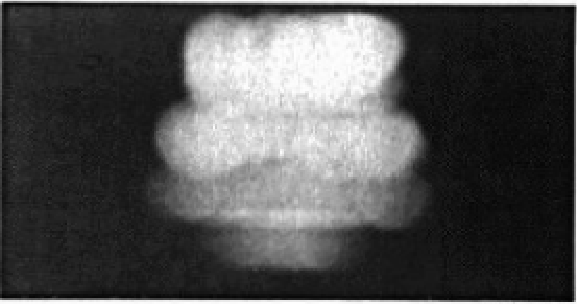
\includegraphics[width=0.25\linewidth]{./figs/hole2mm.pdf}} \hspace{0.08in}
	\subfigure[1mm]
	{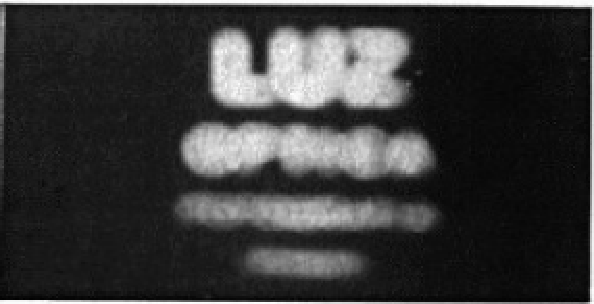
\includegraphics[width=0.25\linewidth]{./figs/hole1mm.pdf}} \\
	\subfigure[0.6mm]
	{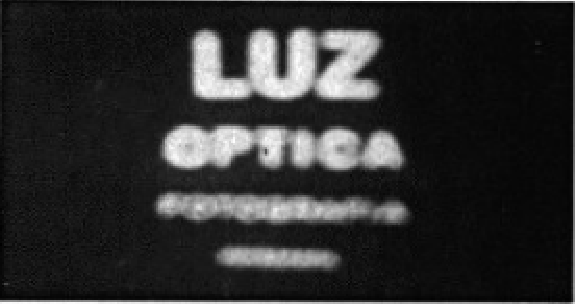
\includegraphics[width=0.25\linewidth]{./figs/hole06mm.pdf}} \hspace{0.08in}
	\subfigure[0.35mm]
	{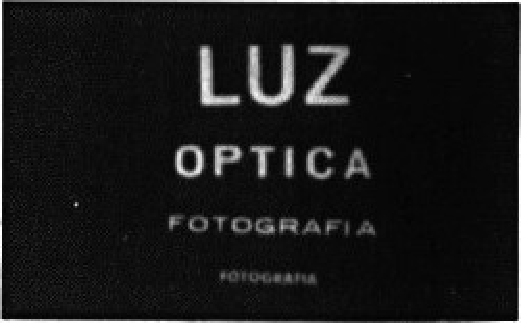
\includegraphics[width=0.25\linewidth]{./figs/hole035mm.pdf}}\\ 
\end{center}
\caption{Imaging with different sizes of hole.}
\end{figure}
\begin{itemize}
	\item {Is it the smaller the better?}
\end{itemize}
\end{frame}

\begin{frame}
 \frametitle{Basic knowledge about camera: the lens (4)}
 \vspace{-0.1in}
\begin{figure}
\begin{center}
	\subfigure[2mm]
	{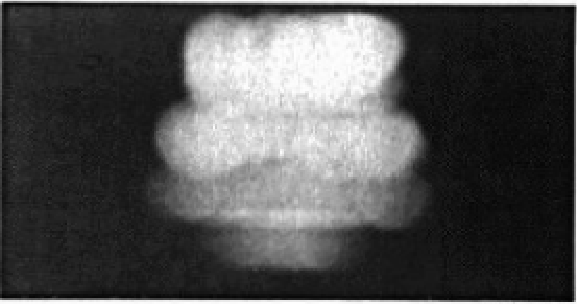
\includegraphics[width=0.25\linewidth]{./figs/hole2mm.pdf}} \hspace{0.08in}
	\subfigure[1mm]
	{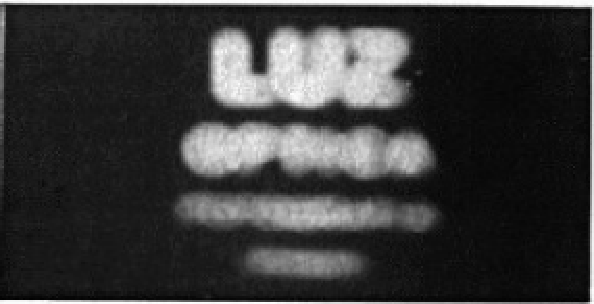
\includegraphics[width=0.25\linewidth]{./figs/hole1mm.pdf}} \\
	\subfigure[0.6mm]
	{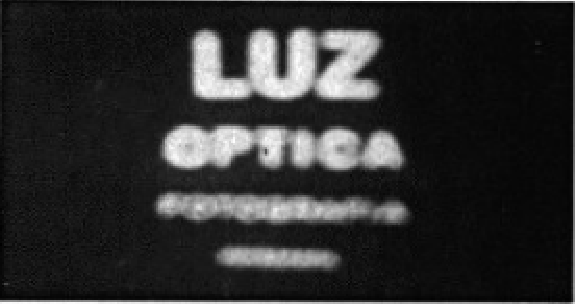
\includegraphics[width=0.25\linewidth]{./figs/hole06mm.pdf}} \hspace{0.08in} 
	\subfigure[0.35mm]
	{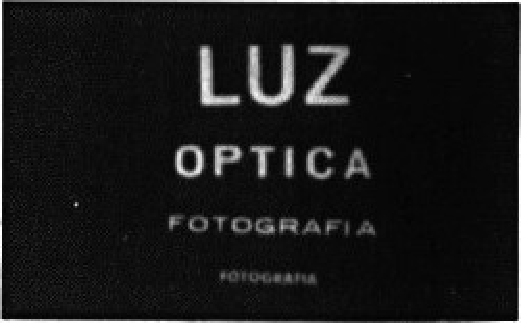
\includegraphics[width=0.25\linewidth]{./figs/hole035mm.pdf}}\\ 
	\subfigure[0.17mm]
	{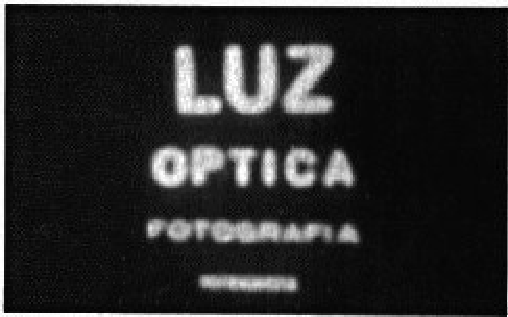
\includegraphics[width=0.25\linewidth]{./figs/hole015mm.pdf}} \hspace{0.08in}
	\subfigure[0.07mm]
	{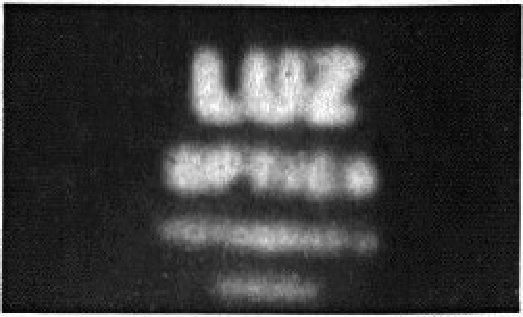
\includegraphics[width=0.25\linewidth]{./figs/hole007mm.pdf}}
\end{center}
\caption{Imaging with different sizes of hole.}
\end{figure}
\end{frame}

%\begin{frame}
% \frametitle{Basic knowledge about camera: the lens (5)}
% \begin{columns}
% \begin{column}{0.6\linewidth}
% \vspace{-0.20in}
%\begin{figure}
%\begin{center}
%	{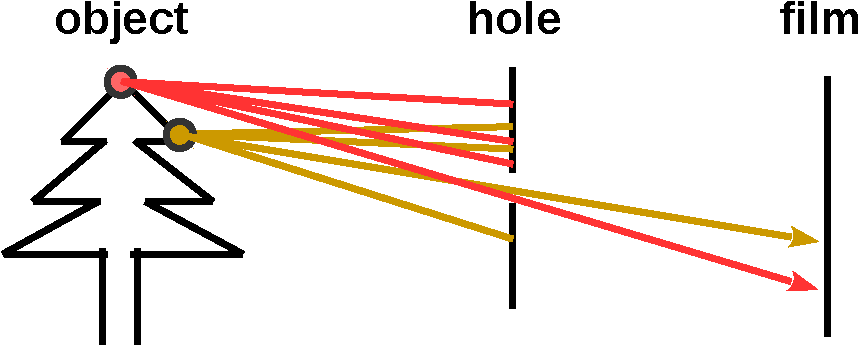
\includegraphics[width=0.9\linewidth]{./figs/hole.pdf}} \\
%	{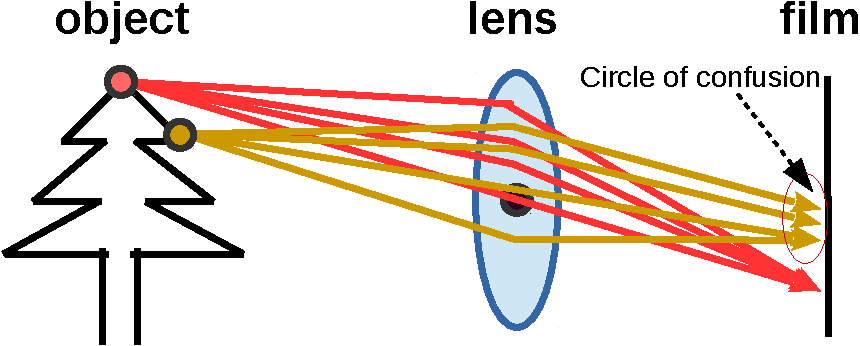
\includegraphics[width=0.9\linewidth]{./figs/lens.pdf}}
%\end{center}
%\caption{Function of the lens.}
%\end{figure}
%\end{column}
%\begin{column}{0.4\linewidth}
%\begin{itemize}
%	\item {Confusion is inevitable}
%	\item {Overall it is beter to integrate lens}
%\end{itemize}
%\end{column}
%\end{columns}
%\end{frame}
%
%\begin{frame}
% \frametitle{Basic knowledge about camera: the aperture (6)}
%\begin{figure}
%\begin{center}
%	{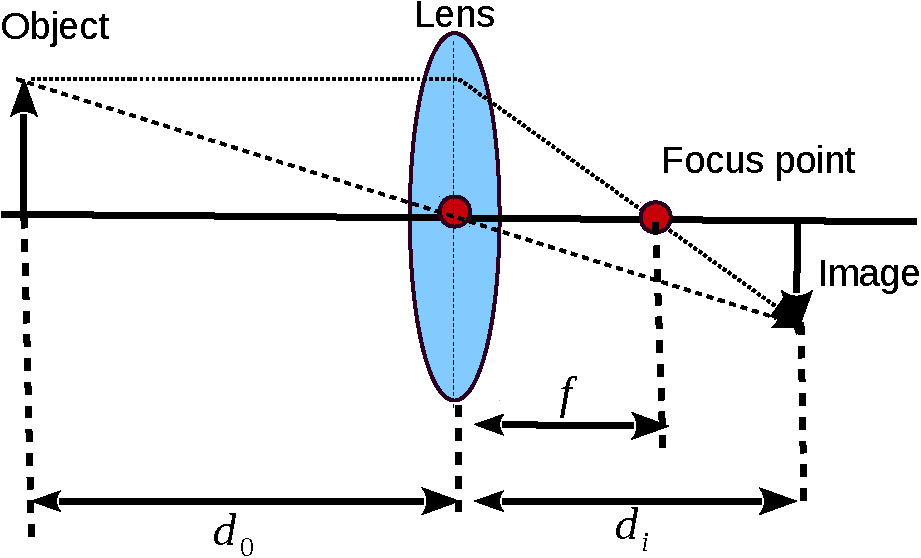
\includegraphics[width=0.6\linewidth]{./figs/lens_strct.pdf}}
%\end{center}
%\end{figure}
%\begin{itemize}
%	\item {We knew following equation in our high school}
%\end{itemize}
%\begin{equation}
%	\frac{1}{d_0}+\frac{1}{d_i}=\frac{1}{f} \nonumber
%\end{equation}
%\begin{itemize}
%	\item {When $d_0$ and $f$ are fixed, $d_i$ cannot be arbitrarily large or small}
%\end{itemize}
%\end{frame}
%
%\begin{frame}
% \frametitle{Basic knowledge about camera: the aperture (7)}
% \begin{itemize}
% 	\item {Previous equation does not hold always in practice}
% \end{itemize}
%\begin{figure}
%\begin{center}
%	\subfigure[]
%	{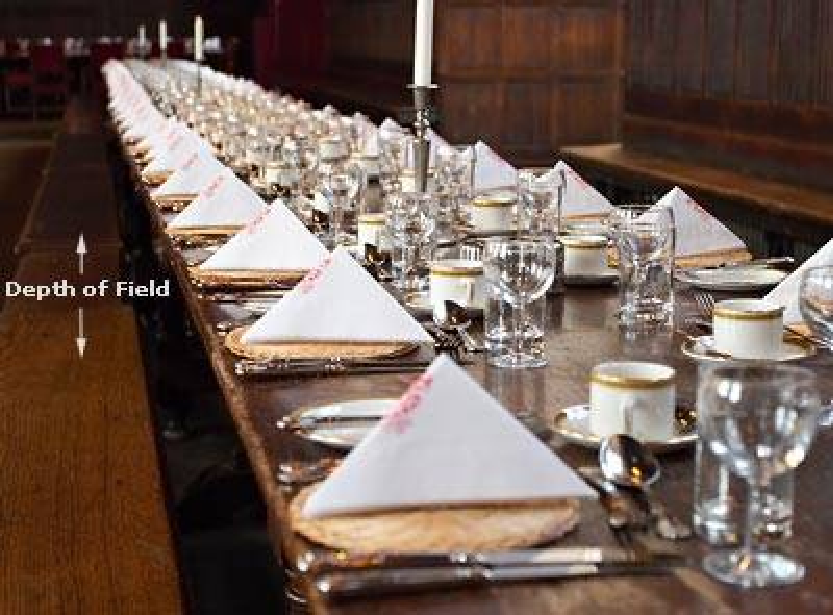
\includegraphics[width=0.48\linewidth]{./figs/depthfield1.pdf}}
%	\subfigure[]
%	{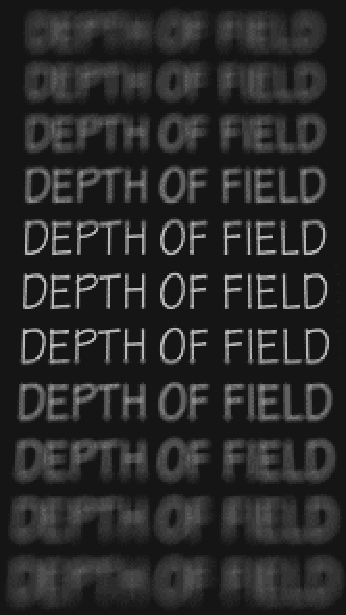
\includegraphics[width=0.20\linewidth]{./figs/depthfield2.pdf}}
%\end{center}
%\end{figure}
%\begin{itemize}
%	\item {Only certain range of ``depth of field'' is clear to us}
%\end{itemize}
%\end{frame}
%
%\begin{frame}
% \frametitle{Basic knowledge about camera: the lens (8)}
%\begin{figure}
%\begin{itemize}
%	\item {The length of focus also plays an important role}
%\end{itemize}
%\begin{center}
%	{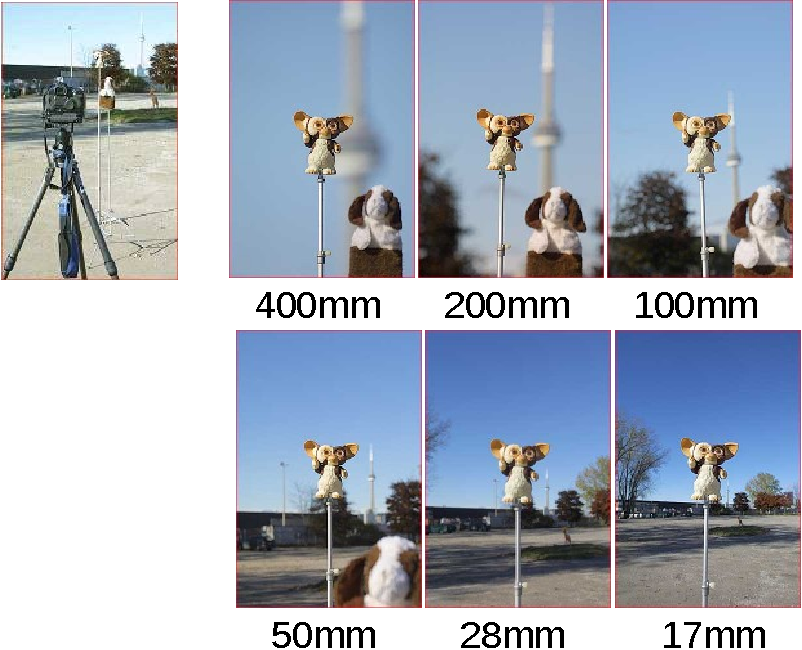
\includegraphics[width=0.5\linewidth]{./figs/longfocus.pdf}} \\
%\end{center}
%\caption{The impact of focus lens, imaging when the length of focus varies.}
%\end{figure}
%\begin{itemize}
%	\item {Large focus length compresses the depth}
%\end{itemize}
%\end{frame}

\begin{frame}
 \frametitle{Basic knowledge about camera: the aperture (1)}
\begin{figure}
\begin{center}
	{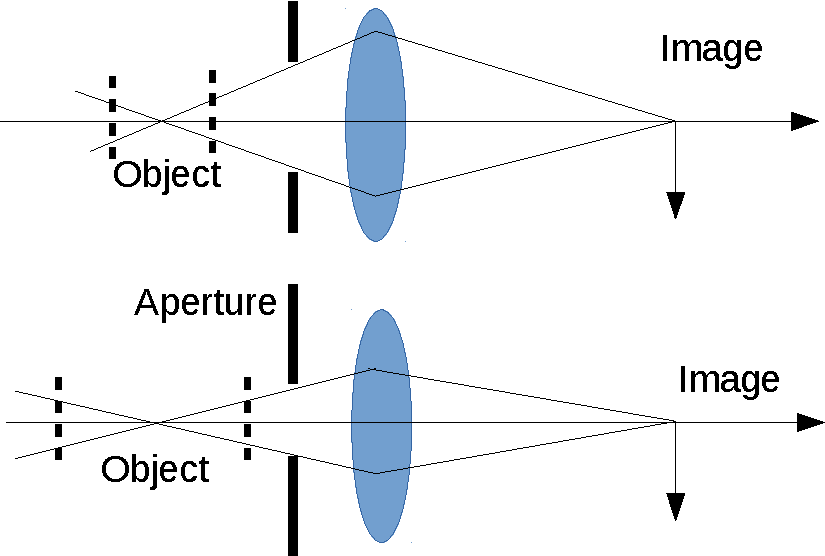
\includegraphics[width=0.55\linewidth]{./figs/apert3.pdf}}
\end{center}
\end{figure}
\begin{itemize}
	\item {Large aperture covers relatively short ``\textbf{depth of field}''}
	\item {Small aperture covers wide ``\textbf{depth of field}'' (DOF)}
	\item {However, small aperture allows less light pass-through}
	\item {It requires longer exposure time}
\end{itemize}
\end{frame}


\begin{frame}
 \frametitle{Basic knowledge about camera: the aperture (2)}
\begin{figure}
\begin{center}
	\subfigure[f=2.8, large aperture]
	{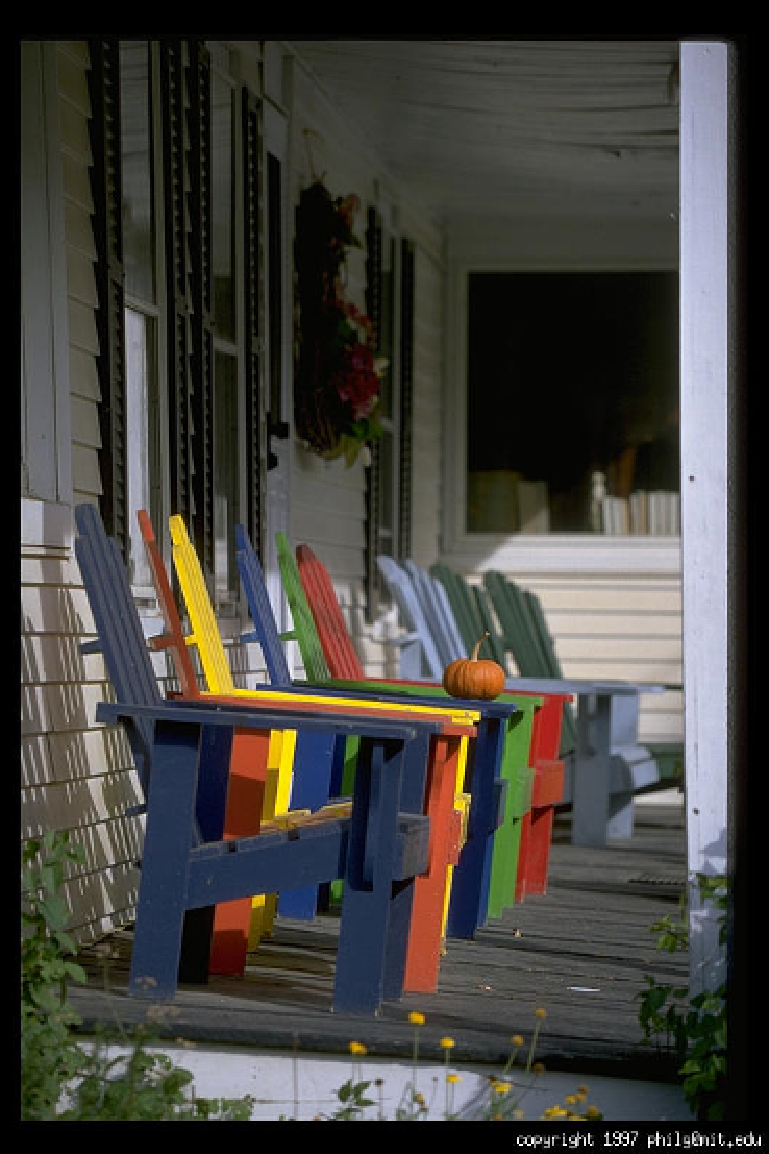
\includegraphics[width=0.30\linewidth]{./figs/apert1.pdf}}
	\hspace{0.15in}
	\subfigure[f=22, small aperture]
	{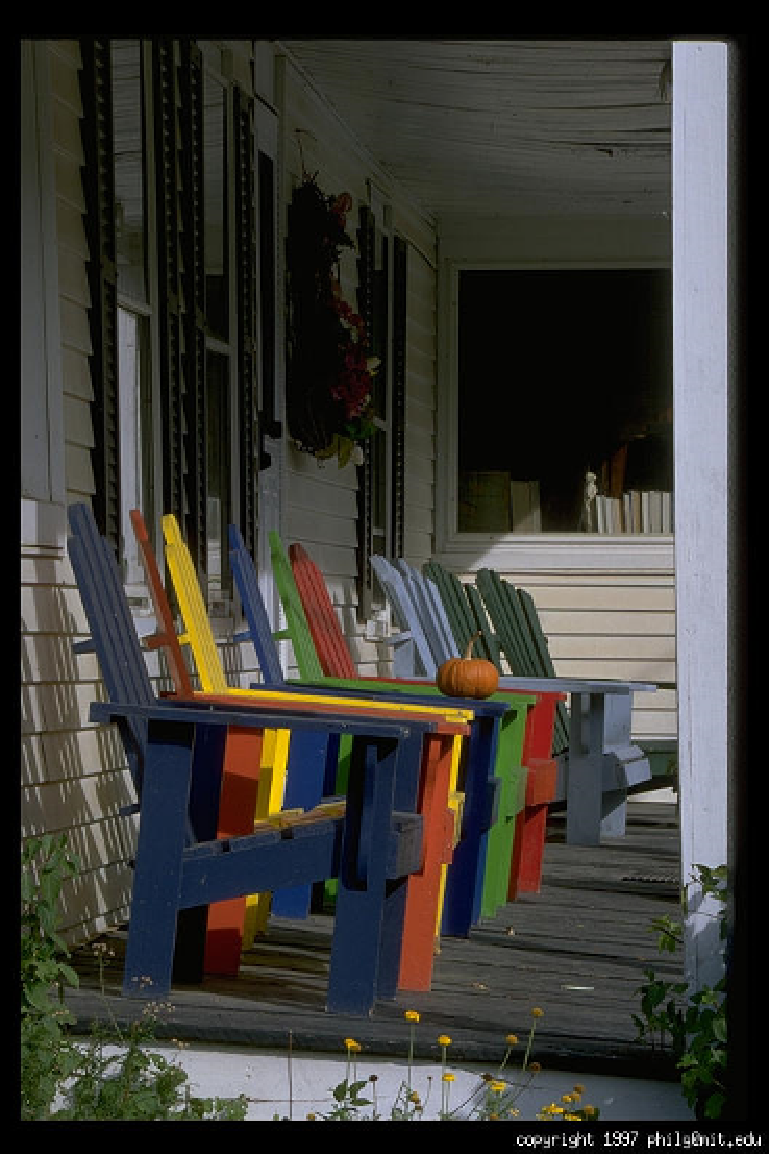
\includegraphics[width=0.30\linewidth]{./figs/apert2.pdf}}
\end{center}
\end{figure}
\begin{itemize}
	\item {Large aperture covers relatively short ``\textbf{depth of field}''}
\end{itemize}
\end{frame}